% !TEX program = xelatex

\documentclass{resume}
\usepackage{graphicx}
% \usepackage{tabu}
\usepackage{booktabs}
\usepackage{multirow}
% \usepackage{progressbar}
\usepackage{hyperref}
% \usepackage{zh_CN-Adobefonts_external} % Simplified Chinese Support using external fonts (./fonts/zh_CN-Adobe/)
% \usepackage{zh_CN-Adobefonts_internal} % Simplified Chinese Support using system fonts

\begin{document}
\pagenumbering{gobble} % suppress displaying page number

\begin{tabular*}{\textwidth}{l c @{\extracolsep{\fill}} r}
  \begin{minipage}{1.4in}
    % adapt widths of minipages to your needs
    % change Large font here
    \textit{
      {\Large \textbf{Gen LI}}                            \\
      48 Rue de la Bourgeon-                              \\
      nière, 44300 Nantes                                 \\
      +33 (0)7 49 99 05 67                                \\
      rami3l@foxmail.com                                  \\
      \href{https://github.com/rami3l}{github.com/rami3l} \\
      Né en février 1999
    }
  \end{minipage} & {
      \renewcommand\arraystretch{1.3}
      \begin{tabular}{c}
        {\LARGE \textbf{Élève Ingénieur - Centrale Nantes}}      \\
        {\Large 2\textsuperscript{ème} Année du Cycle Ingénieur} \\
        {\Large \textbf{Recherche de Stage Ingénieur}}           \\
        {\Large \textbf{(Avril 2022 - 20 semaines)}}
      \end{tabular}
    } &
  \begin{minipage}{1in}
    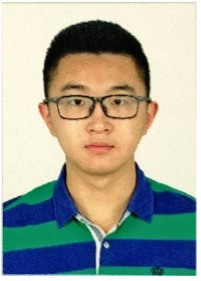
\includegraphics[width=1in]{avatar}
  \end{minipage}
\end{tabular*}


\section{Formation}
\datedsubsection{\textbf{École Centrale de Nantes (ECN)} {\small Nantes, France}}{Depuis Sept. 2020}
\textit{Cycle Ingénieur} (Informatique) : Programme double diplôme avec Centrale Pékin

\datedsubsection{\textbf{Université de Beihang (BUAA) - École Centrale Pékin} {\small Pékin, Chine}}{Sept. 2017 - Juin 2020}
2ème \& 3ème année : Étude des sciences en français (GPA : 3.6647)
\begin{itemize}
  \item Mathématiques, Physique, Science Industrielle, Programmation, …
\end{itemize}
1ère année : Étude intensive de la langue française (générale \& scientifique)

\datedsubsection{\textbf{Lycée Nankai de Chongqing} {\small Chongqing, Chine}}{Sept. 2014 - Juin 2017}
Gaokao (Bac équivalent) : Mention Très Bien (654/750 points)


\section{Expérience professionnelle}
\datedsubsection{\textbf{BUAA} - \href{https://github.com/BUAA-SE-Compiling/rurikawa}{\textit{Rurikawa} : Évaluation des Travaux Pratiques Informatiques}}{Depuis Juin 2020}
Projet en équipe, système de style \textit{Online Judge} automatisant l'évaluation des TP \hfill \textit{Rust, Docker (via Bollard)}
\begin{itemize}
  \item Conception \& réalisation du sous-système d'exécution de code
  \item Contribution à la bibliothèque en amont (\textit{Bollard}, binding de \textit{Docker daemon API} en \textit{Rust})
\end{itemize}

\datedsubsection{\textbf{Projet Personel} - \href{https://github.com/rami3l/pacaptr}{\textit{Pacaptr} : Outil Multiplateforme de Gestion de Paquets}}{Depuis Mars 2020}
Emballage des gestionnaires de paquets utilisant la syntaxe de \textit{pacman} de \textit{Arch Linux} \hfill \textit{Rust, Clap}
\begin{itemize}
  \item Analyse des besoins, réalisation du projet, maintenance continue \& marketing
  \item Utilisation de CI/CD pour la détection des régressions et la distribution des paquets
  \item Contribution à la bibliothèque en amont (\textit{Clap}, bibliothèque \textit{Rust} d'analyse d'arguments CLI)
\end{itemize}

\datedsubsection{\textbf{Projet Personel} - \href{https://github.com/rami3l/yascm}{\textit{Yascm} : Interpréteur simple du langage \textit{Scheme}}}{Depuis Févr. 2020}
Solution à l'un des projets de \textit{SICP} (\textit{Structure and Interpretation of Computer Programs}) \hfill \textit{Haskell, Scala}
\begin{itemize}
  \item Étude de la programmation fonctionnelle et la théorie des langages
  \item Implémentation basé sur l'interpréteur métacirculaire du livre, en \textit{Haskell} et puis en \textit{Scala}
\end{itemize}

\datedsubsection{\textbf{BUAA} - \href{https://github.com/rami3l/CircuitSim}{\textit{CircuitSim} : Simulateur de Circuits Électriques}}{Oct. 2019 – Nov. 2019}
Réalisation d’une version simplifiée de \textit{SPICE}, modélisation orientée objet \hfill \textit{C\#, MathNet}
\begin{itemize}
  \item Coopération \textit{Git} \& gestion des tâches en équipe
\end{itemize}

% Reference Test
%\datedsubsection{\textbf{Paper Title\cite{zaharia2012resilient}}}{May. 2015}
%An xxx optimized for xxx\cite{verma2015large}
%\begin{itemize}
%  \item main contribution
%\end{itemize}

\section{Compétences linguistiques et informatiques}

\begin{tabular}{l l}
  \textbf{Anglais}      & Courant - CET 6    \\
  \textbf{Français}     & Courant - DELF B2  \\
  \textbf{Mandarin}     & Langue Maternelle  \\
  \textbf{Informatique} & Rust, Python, Java
\end{tabular}

% \section{\faHeartO\ Honors and Awards}
% \datedline{\textit{\nth{1} Prize}, Award on xxx }{Jun. 2013}
% \datedline{Other awards}{2015}

\section{Centre d’intérêts et activités}
\begin{tabular*}{\textwidth}{l l @{\extracolsep{\fill}} r}
  \textbf{Engagement Citoyen} & Vélocampus & Depuis Oct. 2020 \\
  \textbf{Activité Sociale} & Étude des Systèmes de Métro - Chengdu \& Chongqing & Août 2018 \\
  \textbf{Loisirs \& Intérêts} & Photographie \& Design
\end{tabular*}

%% Reference
%\newpage
%\bibliographystyle{IEEETran}
%\bibliography{mycite}
\end{document}
